\chapter{Analisi Iniziale delle Prestazioni}

L'ottimizzazione di un titolo in HDRP non può prescindere da una fase di misurazione rigorosa. Prima di applicare le tecniche di \textit{batching} e lo sviluppo di \textit{shader} ottimizzati, è necessario stabilire una metodologia di indagine che permetta di identificare con precisione i colli di bottiglia (\textit{bottleneck}) del sistema.

\section{Presentazione della scena di riferimento}

La scena selezionata per l'analisi delle prestazioni è denominata \textit{Chemical Plant}. Si tratta di un ambiente industriale di vaste dimensioni che alterna ampi spazi aperti a complessi interni strutturati su più livelli. Questa specifica ambientazione è stata scelta poiché integra diverse criticità tecniche che mettono sotto sforzo la \textit{High Definition Rendering Pipeline} (HDRP).

\subsection{Caratteristiche della Scena e Criticità Computazionali}

L'analisi si è focalizzata sui seguenti aspetti strutturali, rappresentativi delle sfide di ottimizzazione affrontate nel progetto:

\begin{itemize}
    \item \textbf{Densità di Asset Modulari:} La scena presenta una massiccia ripetizione di elementi geometrici complessi, quali tubature, valvole e strutture portanti metalliche. Se non gestiti correttamente tramite tecniche di \textit{batching}, tali oggetti generano un numero di \textit{draw call} insostenibile per la CPU.
    \item \textbf{Gestione degli Spazi Aperti:} Negli esterni, l'elevata distanza di rendering (\textit{draw distance}) obbliga il motore a processare un numero ingente di vertici, rendendo critico il sistema di \textit{culling} e la gestione dei \textit{Level of Detail} (LOD).
    \item \textbf{Illuminazione e Riflessioni:} Il contesto industriale richiede l'uso di numerosi \textit{point light} e \textit{spotlight} per simulare l'illuminazione artificiale dei macchinari. Inoltre, la presenza di materiali metallici e superfici con diversi gradi di \textit{smoothness} richiede calcoli intensivi per le riflessioni in tempo reale e le \textit{Shadow Maps}.
\end{itemize}

\begin{figure}[H]
    \centering
    \begin{minipage}{0.48\textwidth}
        \centering
        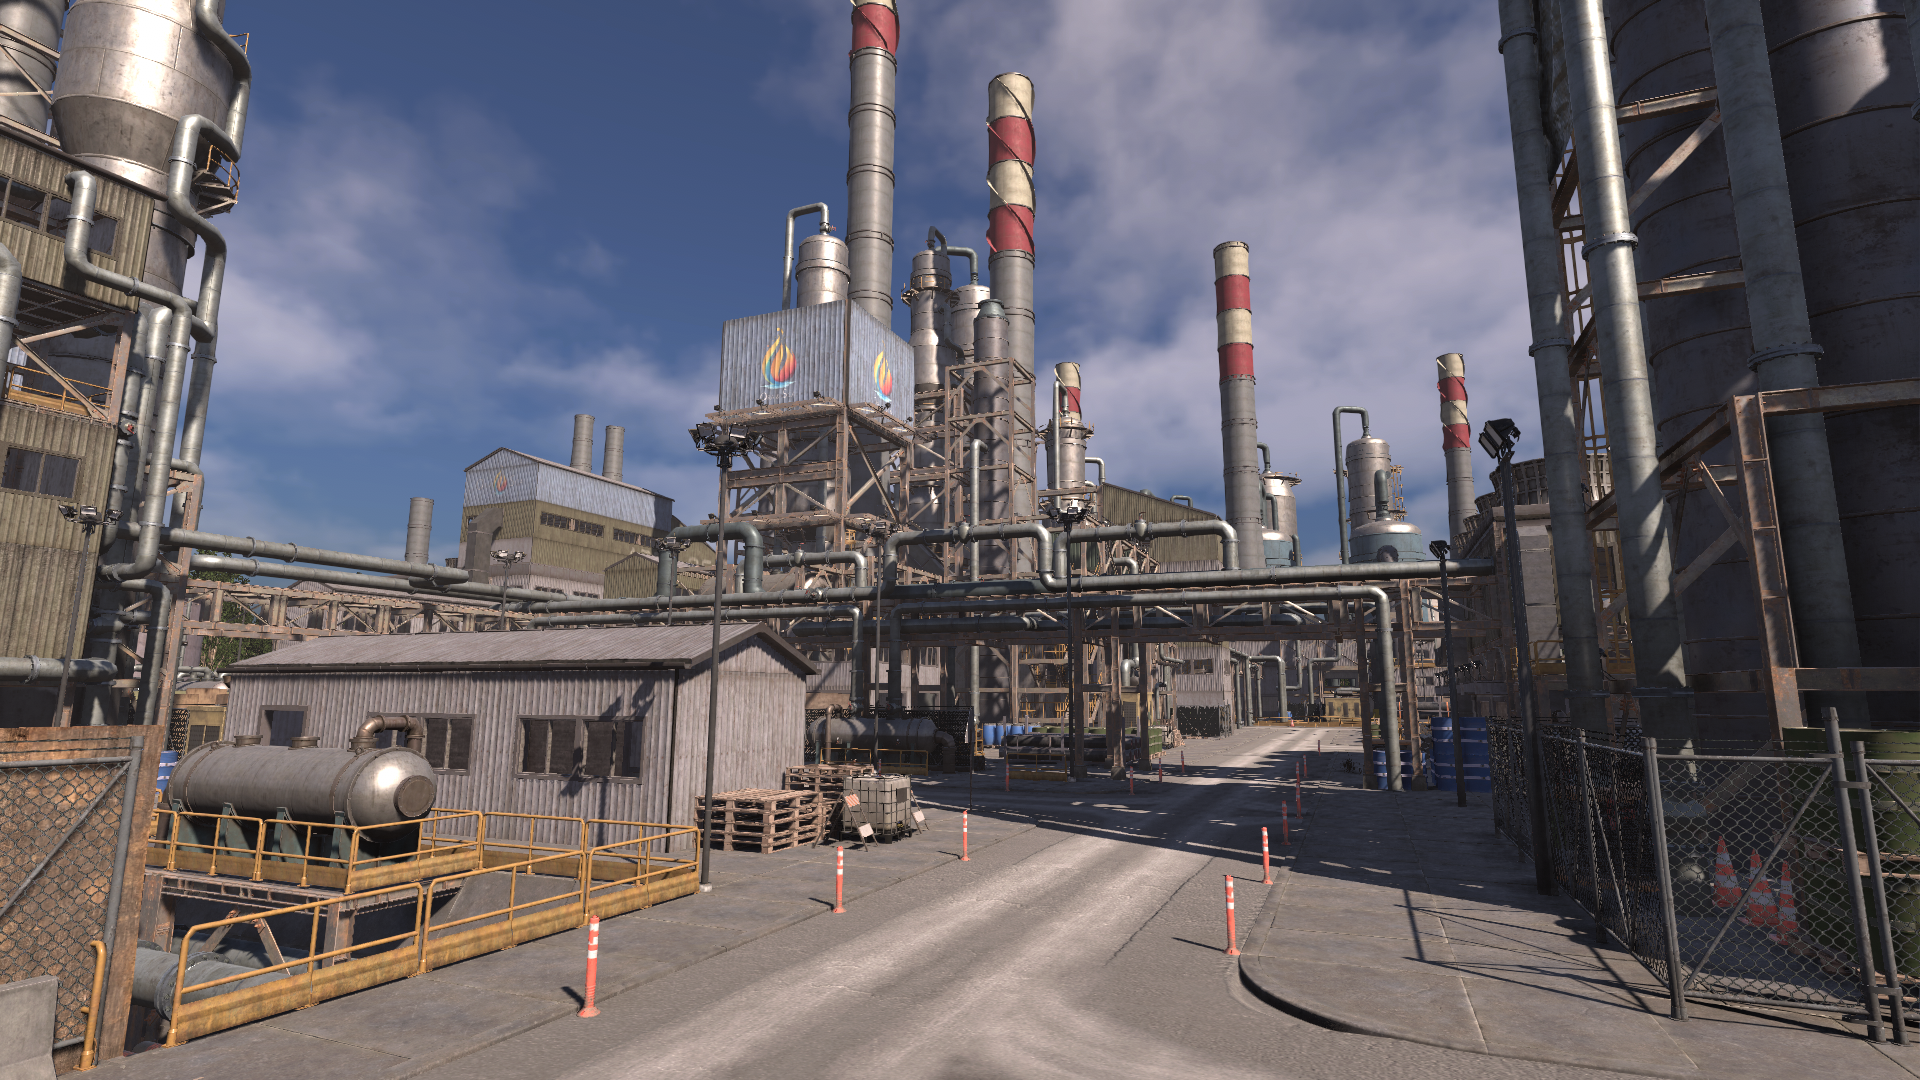
\includegraphics[width=\textwidth]{immagini/cap3/chemical_plant_outdoor.png}
        \caption*{\small (a) Outdoor Environment}
    \end{minipage}
    \hfill
    \begin{minipage}{0.48\textwidth}
        \centering
        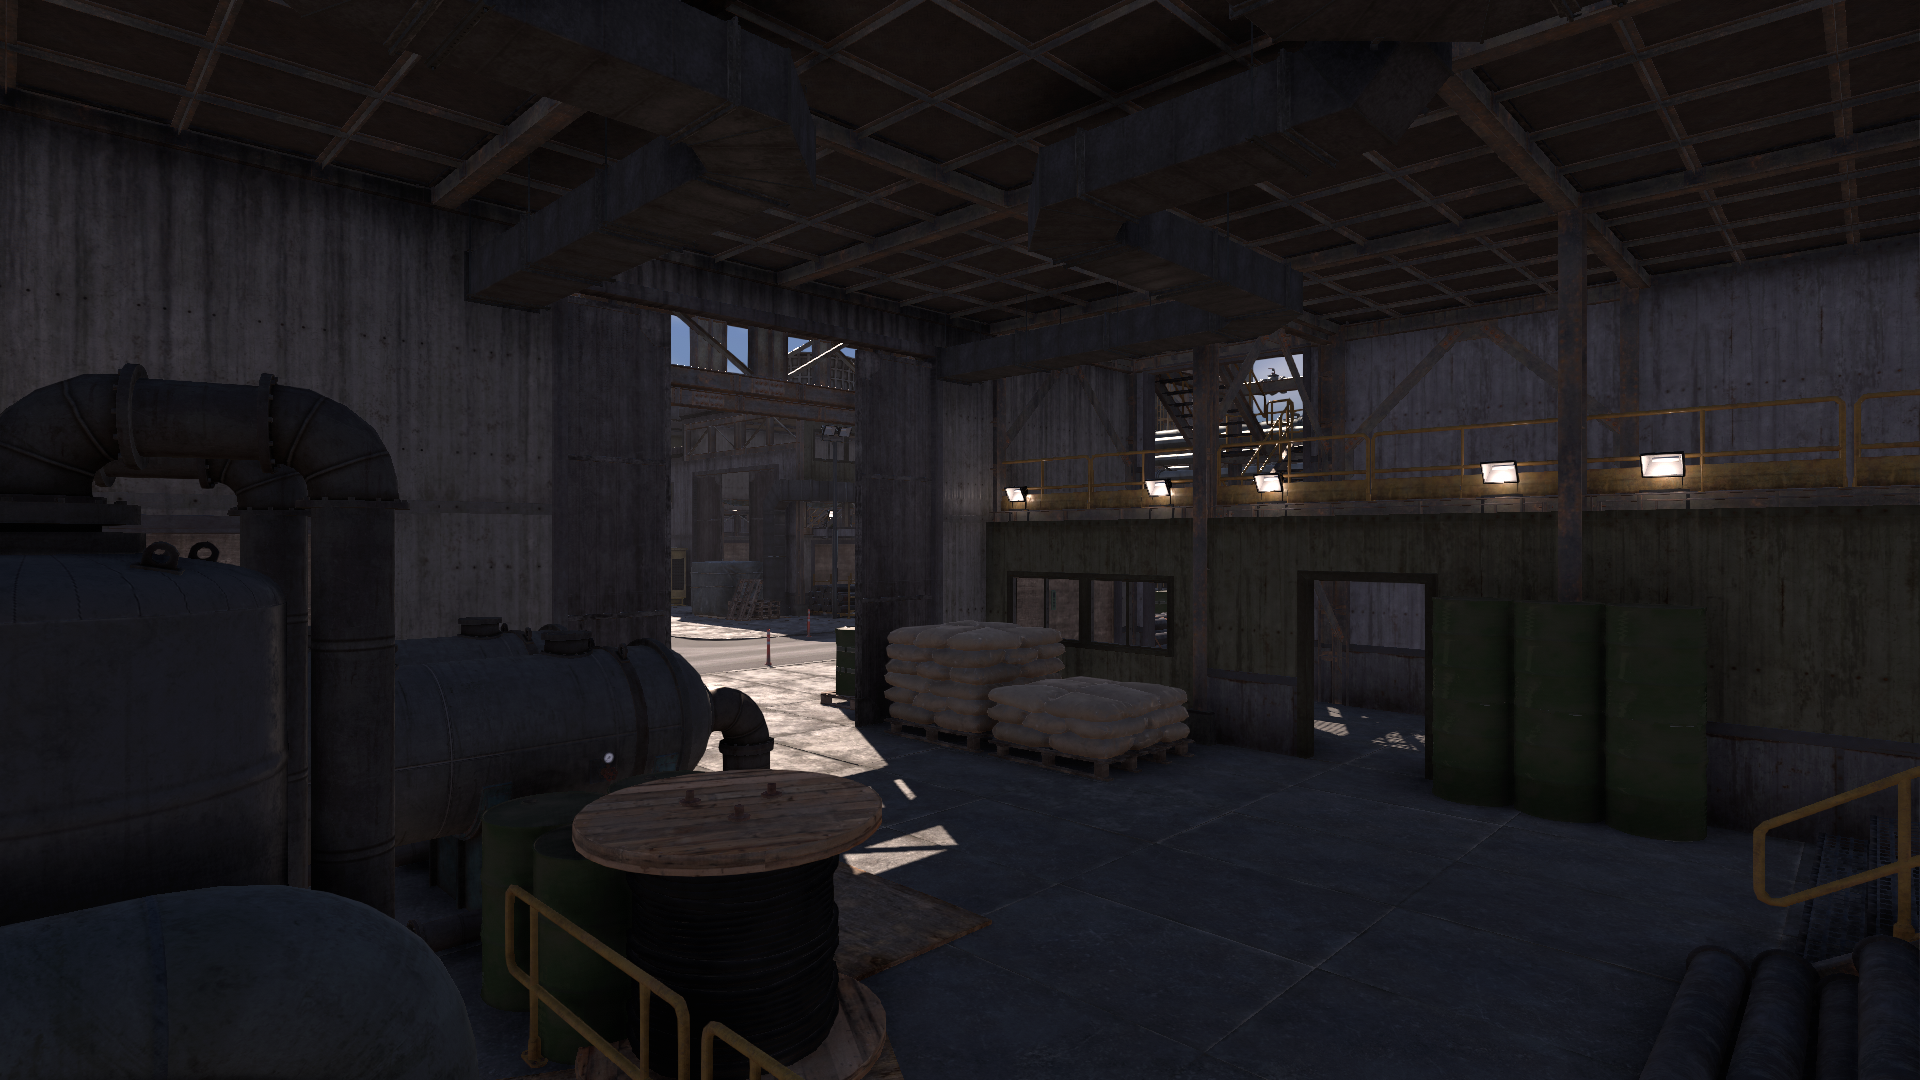
\includegraphics[width=\textwidth]{immagini/cap3/chemical_plant_indoor.png}
        \caption*{\small (b) Indoor Environment}
    \end{minipage}
    \caption{Dettagli della scena "Chemical Plant"}
    \label{fig:chemical_plant_details}
\end{figure}

\section{Strumenti di Profiling}

Per l'analisi quantitativa e qualitativa delle prestazioni di ARES, sono stati utilizzati i \textit{tool} ufficiali integrati nell'ecosistema Unity. Questi strumenti permettono di scindere il carico di lavoro del processore centrale (CPU) da quello della scheda grafica (GPU), identificando con precisione la natura dei colli di bottiglia.

\subsection{Unity Profiler}

L'Unity Profiler è lo strumento di analisi quantitativa fondamentale per monitorare l'allocazione delle risorse hardware in tempo reale. Esso permette di registrare le prestazioni del gioco durante l'esecuzione, fornendo un grafico temporale della durata di ogni singolo \textit{frame} suddiviso per moduli funzionali.

\subsubsection{Struttura e Moduli di Analisi}

L'interfaccia del Profiler è organizzata gerarchicamente per offrire diversi livelli di astrazione:

\begin{itemize}
    \item \textbf{Profiler Modules (Vista Macro):} Situata nella parte superiore, questa sezione mostra grafici a aree relativi a diverse categorie di consumo. Per l'ottimizzazione di ARES, il modulo \textit{Rendering} risulta critico, in quanto riporta il numero di \textit{Draw Calls}, \textit{SetPass Calls} e il tempo totale speso dalla CPU per istruire la pipeline grafica.
    \item \textbf{Timeline View (Vista Micro):} Posizionata nella parte inferiore, questa vista visualizza l'esecuzione parallela dei diversi \textit{thread} del motore. È stata utilizzata per analizzare la sincronizzazione tra il \textbf{Main Thread} e il \textbf{Render Thread}.
\end{itemize}

\begin{figure}[H]
    \centering
    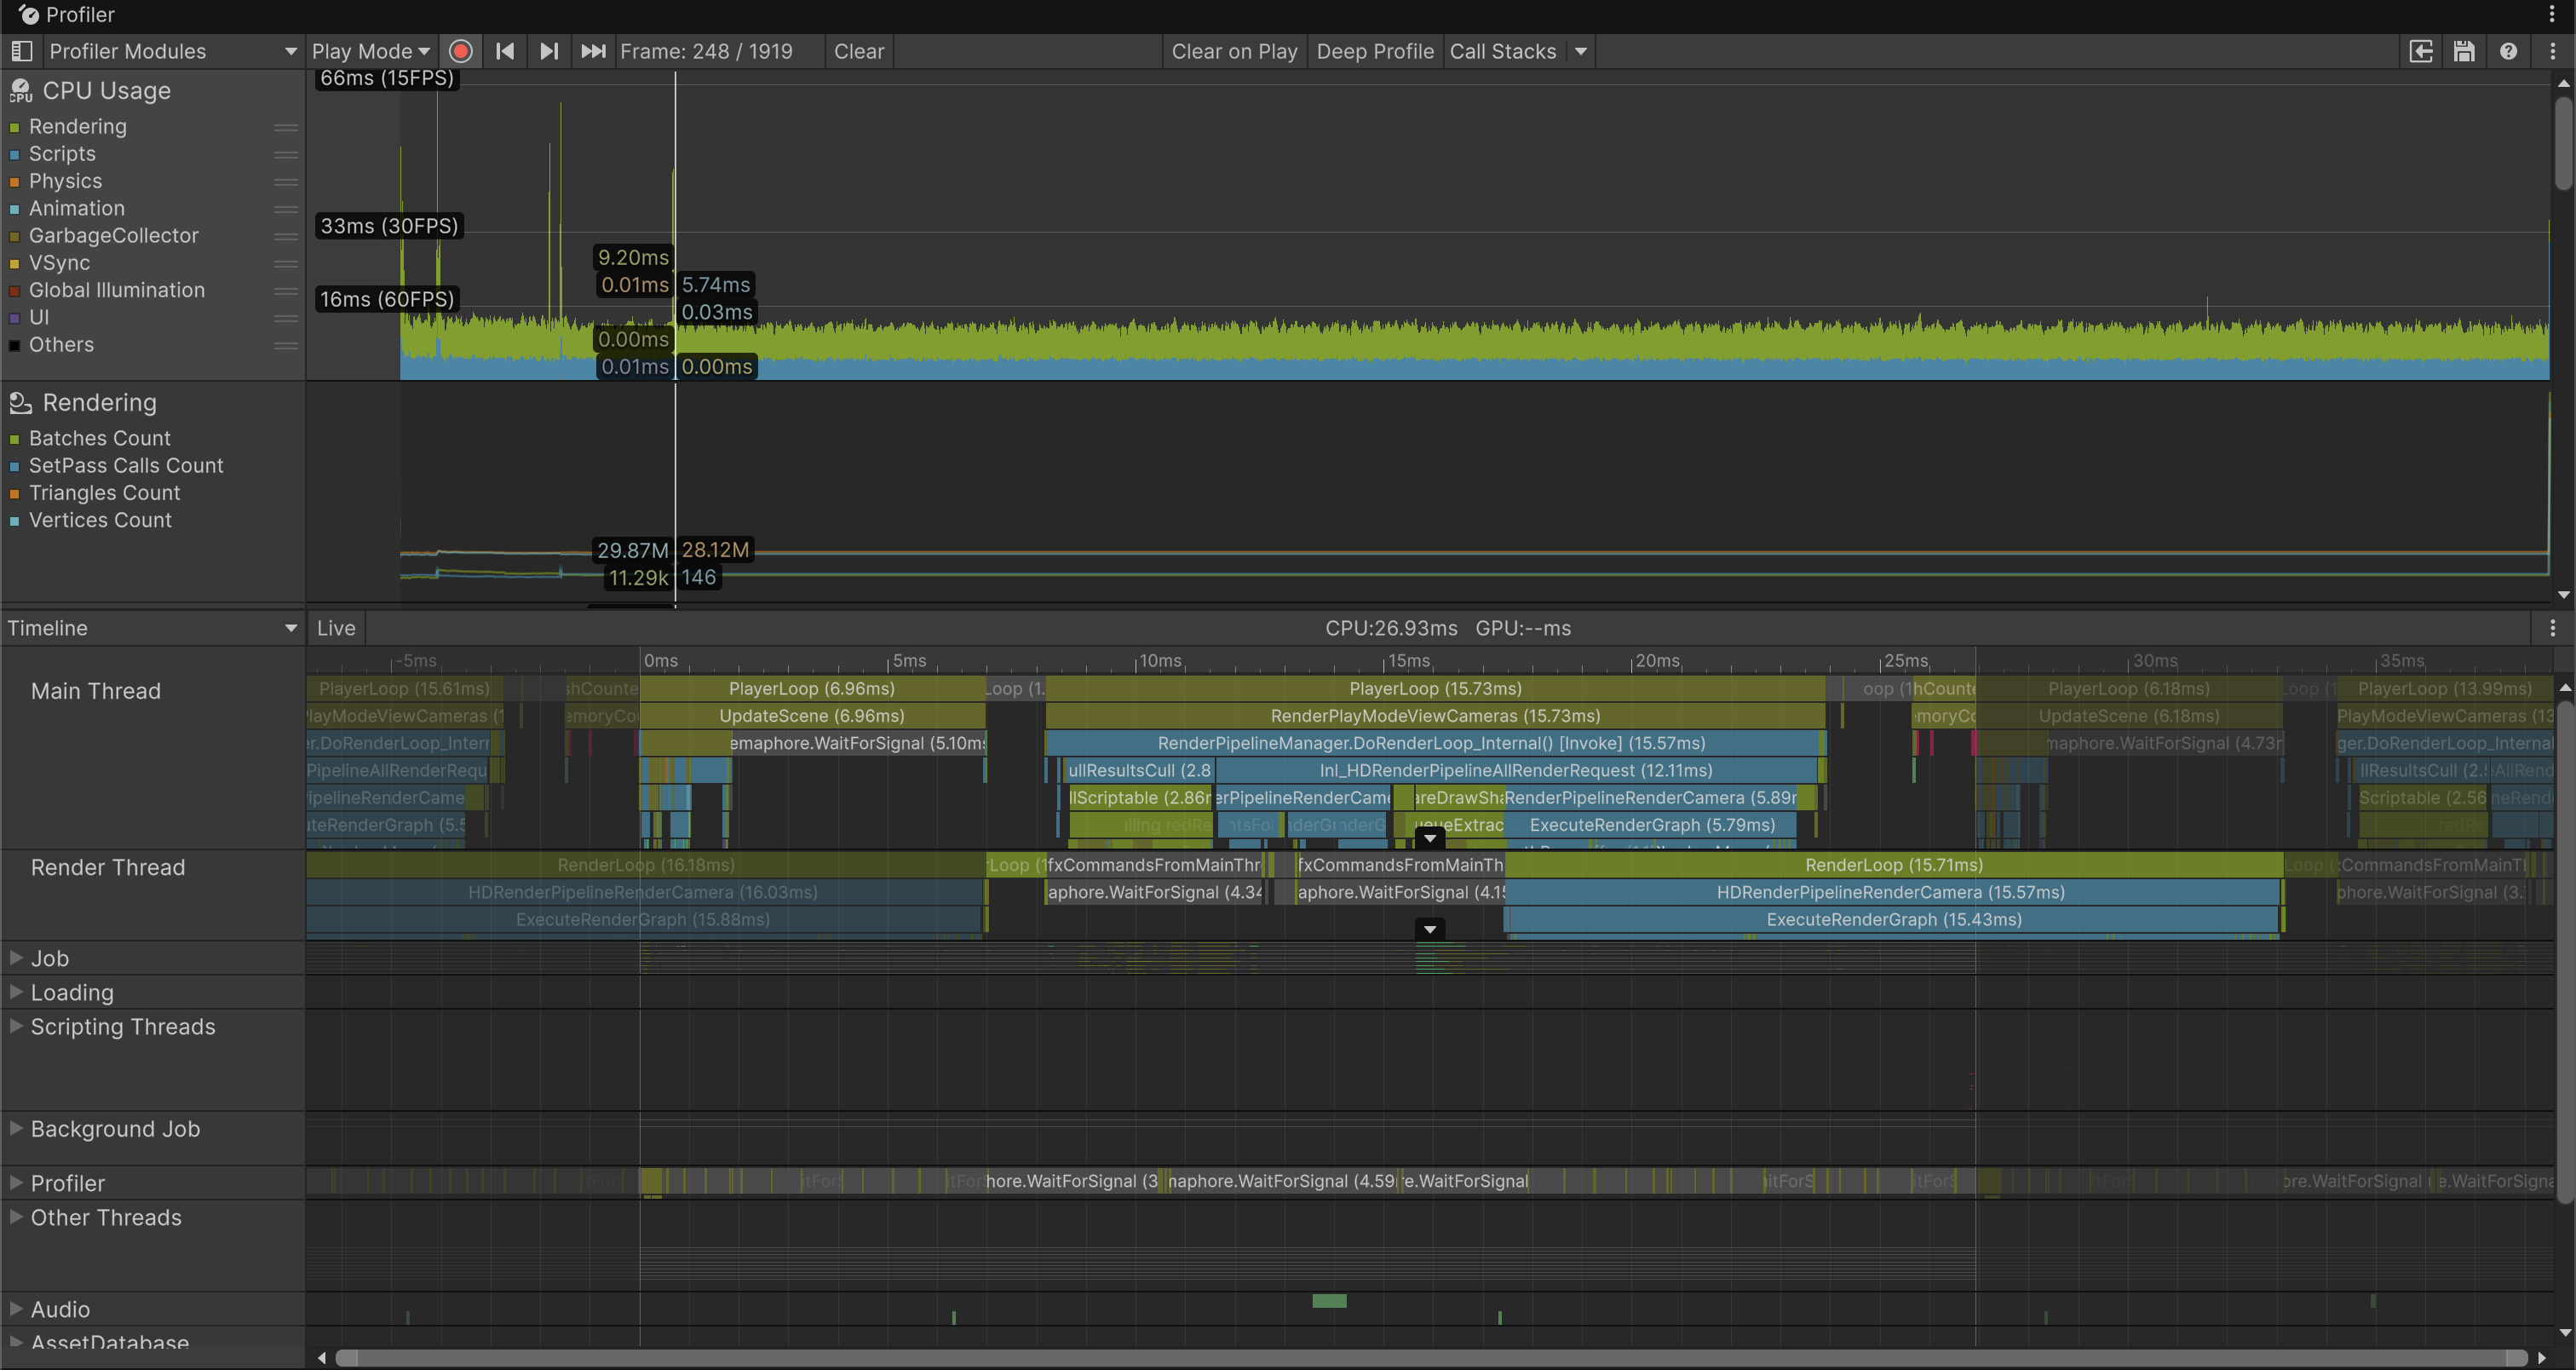
\includegraphics[width=\textwidth]{immagini/cap3/unity_profiler_structure.png}
    \caption{Analisi dettagliata tramite Unity Profiler in modalità Timeline. Nella sezione inferiore è possibile osservare la distribuzione del carico di lavoro tra Main Thread e Render Thread, identificando i tempi di esecuzione delle funzioni di rendering della HDRP.}
    \label{fig:profiler_structure}
\end{figure}

\subsubsection{Metriche Critiche per l'Ottimizzazione}

Prima di procedere con la fase sperimentale, è fondamentale definire le metriche prestazionali che fungeranno da indicatori chiave per valutare l'efficacia degli interventi di ottimizzazione. Queste grandezze, monitorate attraverso i moduli del Profiler, permettono di mappare il carico di lavoro tra i diversi componenti hardware.

Le metriche selezionate per lo studio della scena \textit{Chemical Plant} sono:

\begin{itemize}
    \item \textbf{Batches e SetPass Calls:} I \textit{Batches} indicano il numero di pacchetti di geometria inviati alla GPU per il disegno. Le \textit{SetPass Calls} rappresentano invece quante volte la GPU deve cambiare il proprio stato interno per elaborare un nuovo materiale o shader. Una riduzione di questi valori indica una migliore aggregazione dei dati e un minor carico sulla CPU.
    
    \item \textbf{Frame Time (ms):} Rappresenta il tempo totale impiegato dal sistema per completare tutte le fasi della pipeline. È la metrica principale per determinare la fluidità dell'applicazione, dove tempi inferiori corrispondono a un \textit{frame rate} (FPS) più elevato.
    
    \item \textbf{Triangles e Vertices Count:} Indicano la densità geometrica complessiva processata nel \textit{Vertex Shader}. Monitorare questi valori permette di verificare l'impatto visivo e prestazionale delle tecniche di semplificazione della mesh.
    
    \item \textbf{Gfx.Wait Commands:} Questi marcatori, visibili nella \textit{Timeline View}, indicano i tempi di inattività in cui un thread (Main o Render) rimane in attesa del completamento di un'operazione da parte di un altro componente. L'analisi di questi tempi è essenziale per identificare se il collo di bottiglia risiede nell'elaborazione dei dati (CPU) o nel disegno effettivo dei pixel (GPU).
\end{itemize}

\subsection{Frame Debugger}

Il \textbf{Frame Debugger} è lo strumento fondamentale per l'analisi analitica di ogni singolo fotogramma prodotto dalla pipeline HDRP. A differenza del Profiler, che monitora l'andamento temporale, il Frame Debugger permette di "congelare" il rendering e ispezionare sequenzialmente tutti i comandi inviati dalla CPU alla GPU (\textit{Draw Calls}).

L'utilizzo di questo strumento nella scena \textit{Chemical Plant} ha permesso di:
\begin{itemize}
    \item \textbf{Analizzare la gerarchia del rendering:} Osservare l'ordine cronologico con cui gli oggetti vengono processati, dalla fase di \textit{Depth Prepass} fino al \textit{Post-processing}.
    \item \textbf{Diagnosticare le interruzioni dei batch:} Identificare le cause specifiche che impediscono al motore di raggruppare più oggetti in un'unica operazione di disegno.
    \item \textbf{Verificare gli stati della pipeline:} Controllare quali shader sono attivi per ogni oggetto e come i dati fluiscono attraverso i blocchi programmabili descritti precedentemente.
\end{itemize}

\begin{figure}[H]
    \centering
    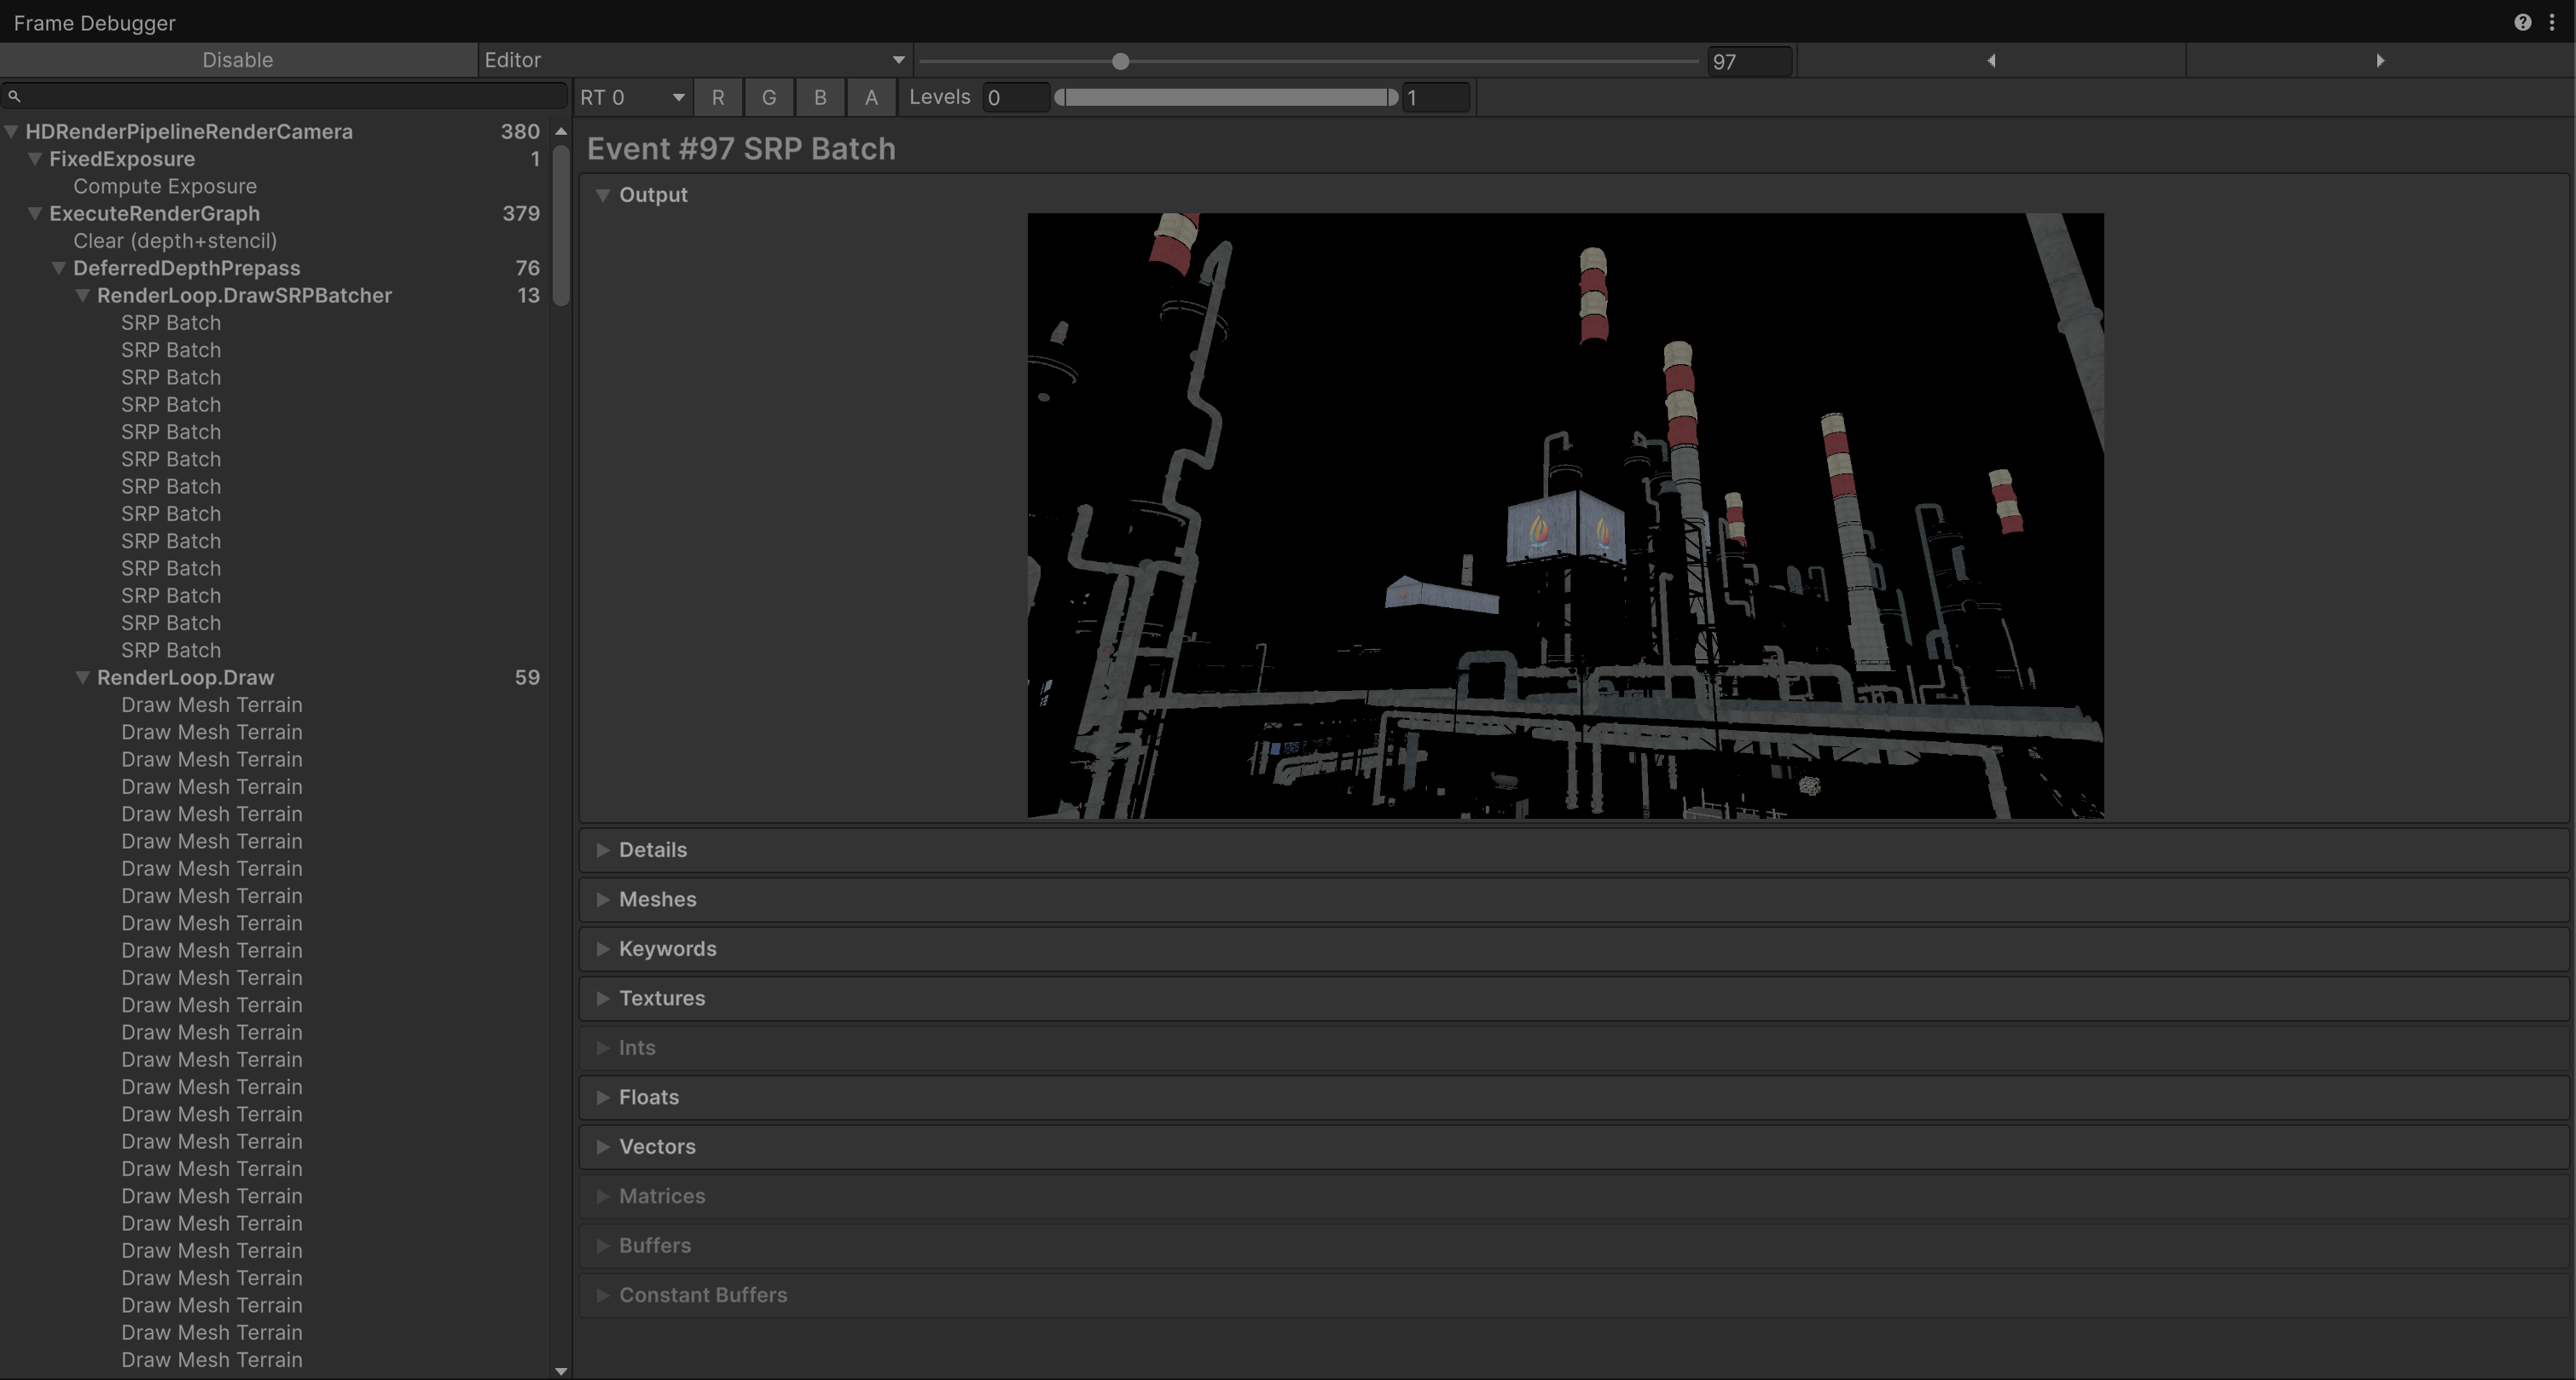
\includegraphics[width=\textwidth]{immagini/cap3/frame_debugger.png}
    \caption{Analisi della scena Chemical Plant tramite Frame Debugger. È possibile osservare la suddivisione delle operazioni di rendering, con particolare evidenza sulle numerose istanze di "Draw Mesh" che non vengono ancora aggregate efficacemente, contribuendo all'elevato numero di draw call totali.}
    \label{fig:frame_debugger}
\end{figure}

\section{Rilevazione della Baseline}

Il processo di analisi ha inizio con la determinazione della \textit{baseline} prestazionale, ovvero la misurazione dello stato del progetto prima di ogni intervento correttivo. Per garantire l'oggettività e la riproducibilità dei dati, la raccolta è stata effettuata attraverso l'impiego di una cinematica fissa. Questo approccio permette di analizzare carichi computazionali identici in ogni sessione di test, rendendo i dati confrontabili tra le diverse iterazioni del processo di ottimizzazione.

\subsection{Setup Sperimentale e Condizioni di Test}

Le rilevazioni sono state condotte su un'unica configurazione hardware di riferimento per isolare le variabili prestazionali legate esclusivamente al motore grafico. Il sistema utilizzato è un \textbf{MacBook Pro} equipaggiato con chip \textbf{Apple M2 Pro}.

Al fine di sottoporre la pipeline HDRP a uno stress test significativo, le impostazioni del motore sono state configurate come segue:
\begin{itemize}
    \item \textbf{Risoluzione:} 1920x1080 (Full HD).
    \item \textbf{Preset di Qualità:} Ultra (impostazioni massime previste dalla HDRP).
    \item \textbf{Metodologia:} Profiling in tempo reale durante l'esecuzione della cinematica fissa.
\end{itemize}

\subsection{Analisi Quantitativa delle Metriche di Rendering}

I dati raccolti evidenziano uno stato di forte inefficienza della pipeline, con valori che superano le soglie ottimali per il target hardware individuato. Di seguito vengono analizzate le metriche fondamentali registrate nei punti di maggiore criticità del percorso.

\subsubsection{Geometria ed Efficienza dei Batch}

L'analisi combinata del carico geometrico e della gestione delle chiamate al disegno rivela le principali criticità che gravano sia sulla CPU che sulla GPU:

\begin{itemize}
    \item \textbf{Complessità Geometrica:} La scena presenta un volume di \textbf{28.13 M di triangoli} e \textbf{29.85 M di vertici}. Tale densità poligonale risulta eccessiva per le reali necessità visive, saturando la pipeline già nella fase di \textit{Vertex Shading} e appesantendo inutilmente la fase di rasterizzazione.
    \item \textbf{Frammentazione delle Draw Calls (11.20 k Batches):} Questo valore rappresenta il principale collo di bottiglia del sistema. Un numero di batch così elevato genera un \textit{overhead} insostenibile per il \textit{Render Thread}, indicando una comunicazione inefficiente tra il processore e la scheda video.
    \item \textbf{Cambi di Stato (146 SetPass Calls):} Sebbene meno critico del batch count, il numero di \textit{SetPass Calls} conferma una mancata standardizzazione dei materiali e degli shader, che interrompe frequentemente la sequenza di invio dei comandi alla GPU.
\end{itemize}

\begin{figure}[H]
    \centering
    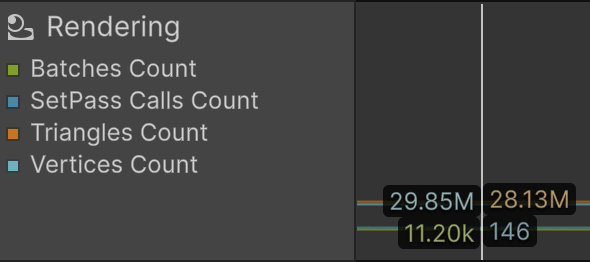
\includegraphics[width=0.9\textwidth]{immagini/cap3/profiler_rendering_baseline.png}
    \caption{Rilevazione dei parametri critici tramite Unity Profiler: si noti l'impatto combinato dell'elevata densità poligonale e degli 11.20k batches sul tempo di frame.}
    \label{fig:profiler_metrics_baseline}
\end{figure}

\subsubsection{Profiling della Timeline}

Per isolare con precisione la causa della bassa frequenza di aggiornamento, è stata effettuata un'analisi granulare del singolo fotogramma attraverso la \textit{Timeline View} del Profiler. Lo \textit{screenshot} riportato in Figura \ref{fig:profiler_timeline_frame} illustra la sequenza temporale delle operazioni eseguite dai thread principali durante un frame rappresentativo della baseline, con un tempo di calcolo complessivo di $32.59\text{ ms}$ (corrispondenti a circa $30\text{ FPS}$).

\begin{figure}[H]
    \centering
    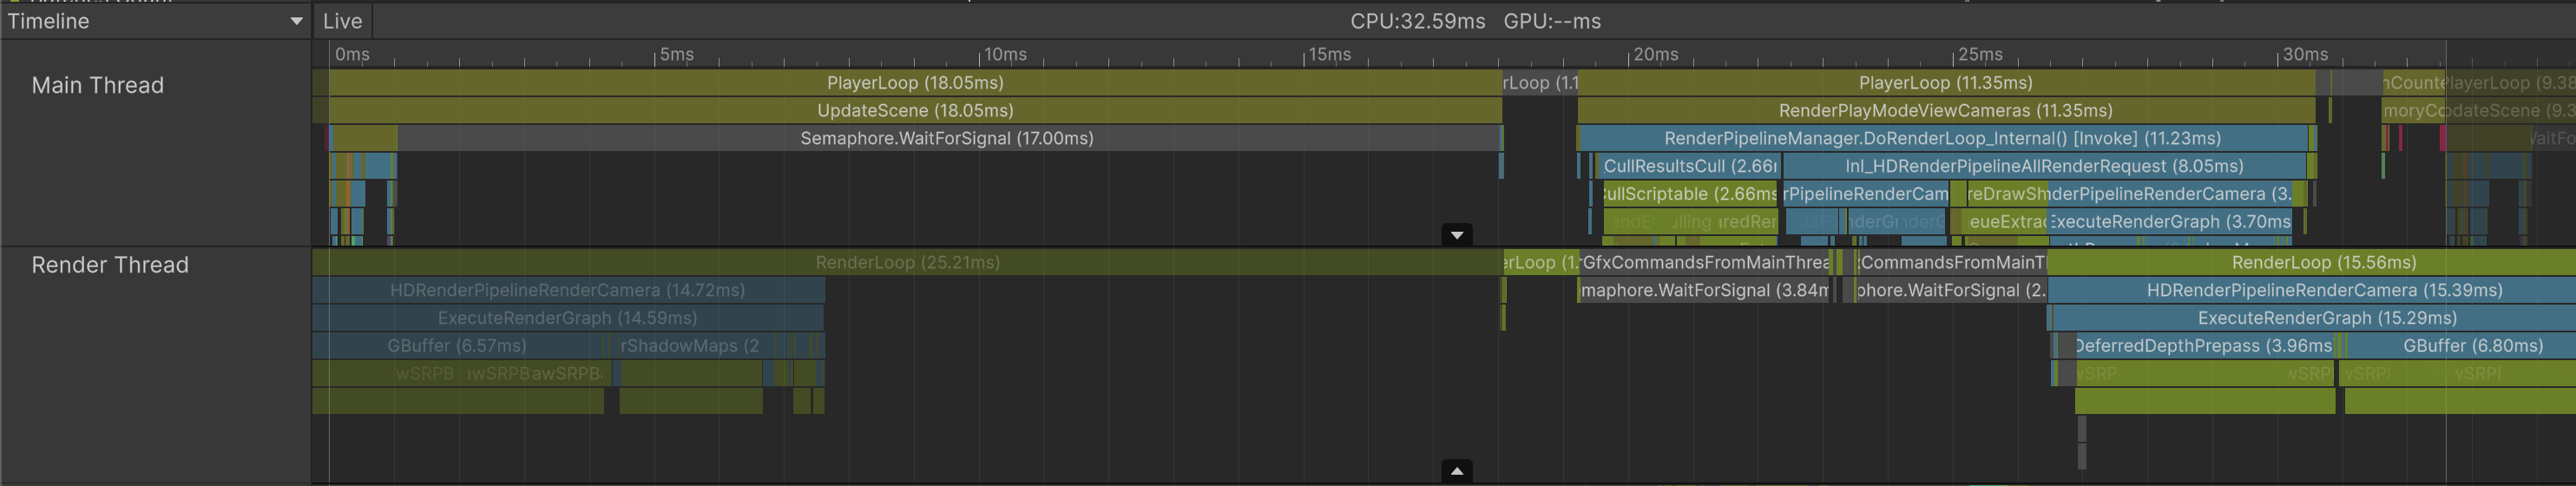
\includegraphics[width=\textwidth]{immagini/cap3/profiler_timeline_baseline.png}
    \caption{Dettaglio della Timeline View: analisi della sincronizzazione tra Main Thread e Render Thread in un singolo fotogramma.}
    \label{fig:profiler_timeline_frame}
\end{figure}

L'ispezione della Timeline permette di scomporre il lavoro del motore e identificare i seguenti problemi strutturali:

\begin{itemize}
    \item \textbf{Stallo del Main Thread (Semaphore):} L'evidenza più significativa è rappresentata dal blocco denominato \textit{Semaphore.WaitForSignal}, che occupa ben $17.00\text{ ms}$ del tempo totale. Sebbene il processore abbia completato la logica di gioco (\textit{PlayerLoop}), esso rimane inattivo in attesa che il \textit{Render Thread} termini l'elaborazione del fotogramma precedente. Questo fenomeno indica che il sistema è \textbf{Render-Thread bound}.
    
    \item \textbf{Sovraccarico del Render Thread:} Il \textit{Render Thread} mostra un \textit{RenderLoop} estremamente esteso ($25.21\text{ ms}$). Al suo interno, la funzione \textit{ExecuteRenderGraph} è rallentata dalla mole spropositata di istruzioni prodotte dagli oltre 11.000 batch. Il thread di rendering agisce come un collo di bottiglia: dovendo "impacchettare" migliaia di piccole chiamate singole per la GPU, non riesce a liberare il \textit{Main Thread} in tempi utili per il fotogramma successivo.
    
    \item \textbf{Culling:} All'interno del \textit{Main Thread}, la fase di \textit{CullResults.Cull} ($2.86\text{ ms}$) risulta proporzionalmente onerosa. Unity deve testare la visibilità di migliaia di oggetti individuali.
    
    \item \textbf{Passaggi HDRP (G-Buffer e Shadow Maps):} Nella parte terminale della sequenza, si osservano i tempi dedicati al \textit{Deferred Depth Prepass} e alla scrittura del \textit{G-Buffer}. L'estensione di questi blocchi conferma che l'alta densità poligonale (28M di triangoli) e la gestione delle ombre proiettate contribuiscono ulteriormente a dilatare il tempo di esecuzione del comando di disegno finale.
\end{itemize}

In sintesi, l'analisi della baseline dimostra che il vero problema non risiede nella potenza della scheda video, ma nella comunicazione tra i componenti del motore. Il sistema impiega troppo tempo nella fase di organizzazione dei dati: il \textbf{Render Thread} è letteralmente sommerso da migliaia di istruzioni individuali e non riesce a "dire" alla GPU cosa disegnare in tempi rapidi. 

Questo genera un effetto a catena che blocca l'intero processo, costringendo il processore a lunghe attese inutili. Risulta quindi evidente che la priorità assoluta per l'ottimizzazione sia l'implementazione di un \textbf{batching} più efficiente, capace di raggruppare questi migliaia di piccoli comandi in pochi blocchi più grandi e gestibili.